\documentclass{../UTNetLab}

\title{Network Management and Security}
\newcommand\reference{
   S. Panwar, S. Mao, J.-dong Ryoo, and Y. Li, “Network management and security,” in TCP/IP Essentials: A Lab-Based Approach, Cambridge: Cambridge University Press, 2004, pp. 187–213.
}

\begin{document}
\part{SNMP Exercises}
    For the exercises in this section, the network topology is given in \hyperref[fig:1.3]{Figure~1.3}, where all the hosts are connected in a single network segment using their IP addresses, i.e.\  from 128.238.66.100 to 128.238.66.102.

    \begin{center}
        \begin{minipage}{0.48\textwidth}
            \begin{flushleft}
                \begin{table}[H]
                    \caption{The IP addresses of the hosts (Table~1.2)}
                    \centering
                    \begin{tabular}{ c c c }
                        \hline \hline
                        Host & IP Address & Subnet Mask \\
                        \hline 
                        h0 & 128.238.66.100 & 255.255.255.0 \\
                        h1 & 128.238.66.101 & 255.255.255.0 \\
                        h2 & 128.238.66.102 & 255.255.255.0 \\
                        h3 & 128.238.66.103 & 255.255.255.0 \\
                        h4 & 128.238.66.104 & 255.255.255.0 \\
                        h5 & 128.238.66.105 & 255.255.255.0 \\
                        h6 & 128.238.66.106 & 255.255.255.0 \\
                        h7 & 128.238.66.107 & 255.255.255.0 \\
                        \hline \hline
                        \end{tabular}
                \end{table}
            \end{flushleft}
        \end{minipage}
        \begin{minipage}{0.48\textwidth}
            \begin{flushright}
                \begin{figure}[H]
                    \centering
                    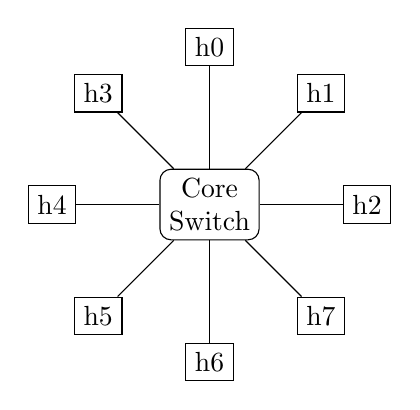
\begin{tikzpicture}
                        \node[draw,align=center,rounded corners] (s) at (0,0){Core\\Switch};
                        \node[draw] (h0) at (0,2){h0};
                        \node[draw] (h1) at ({sqrt(2)},{sqrt(2)}){h1};
                        \node[draw] (h2) at (2,0){h2};
                        \node[draw] (h3) at (-{sqrt(2)},{sqrt(2)}){h3};
                        \node[draw] (h4) at (-2,0){h4};
                        \node[draw] (h5) at (-{sqrt(2)},-{sqrt(2)}){h5};
                        \node[draw] (h6) at (0,-2){h6};
                        \node[draw] (h7) at ({sqrt(2)},-{sqrt(2)}){h7};
                    
                        \draw (h0) -- (s);
                        \draw (h1) -- (s);
                        \draw (h2) -- (s);
                        \draw (h3) -- (s);
                        \draw (h4) -- (s);
                        \draw (h5) -- (s);
                        \draw (h6) -- (s);
                        \draw (h7) -- (s);
                    \end{tikzpicture}
                    \caption{A single segment network (Figure~1.3)}\label{fig:1.3}
                \end{figure}
            \end{flushright}
        \end{minipage}
    \end{center}

    Before the lab, you should:
    \begin{enumerate}
        \item Backup the original \lstinline{snmpd} configuration file:
        \lstinline{mv /etc/snmp/snmpd.conf /etc/snmp/snmpd.conf.save}.
        \item Create a simple configuration file \path{/etc/snmp/snmpd.conf} with a single line defining a read-only community \textbf{guest}:
        \begin{lstlisting}[language={conf}, emph={guest}]
rocommunity guest
        \end{lstlisting}
    \end{enumerate}

\section{SNMP Service and MIB Struct}
    Use \lstinline{pgrep snmpd} to check if \lstinline{snmpd} is started.
    Try to stop and then start the SNMP agent daemon using \lstinline{service snmpd start|stop}.

    Study the \lstinline{snmpd} configuration file \path{/etc/snmp/snmpd.conf}.
    Also study the default configuration file \path{/etc/snmp/snmpd.conf.save}.
    This file is well commented.
    Read the comments and study the configuration options.

    Study the MIB files in the \path{/usr/share/snmp/mibs} directory.
    Examine the Interface MIB \path{IF-MIB.txt} and the TCP MIB \path{TCP-MIB.txt} to see the MIB objects and data types.
    Save these two files for the lab report.

    \begin{report}
    \item What is the community name used in this lab? What is the use of the
    community name?
    
    \item What is the data type for the MIB object \texttt{ifMtu.2}? What is the definition of the MIB object \texttt{ifPhysAddress} and \texttt{ifInOctets}?
    
    \item What is the data type and definition of \texttt{tcpRtoAlgorithm}? What values are allowed for \texttt{tcpRtoAlgorithm}? What is the definition of \texttt{tcpMaxConn}?
    \end{report}

\section{SNMP List Objects}
    Use \lstinline[emph=guest]{snmpwalk -v 2c -c guest localhost interface} to display the Interface MIB.

    Use \lstinline[emph=guest]{snmpwalk -v 2c -c guest localhost tcp} to display the TCP MIB.

    You may run \lstinline{man snmpwalk} to find out the meanings of the options used in the commands.
    Compare the outputs with the MIB files you saved in the previous exercise.
    Also compare the outputs of the first command with that of \lstinline{ifconfig -a}.

    Retry the \lstinline{snmpwalk} commands, but change \textbf{guest} to \textbf{public}.
    Can you display the MIBs this time?
    
    \begin{report}
    \item What is the MTU of the Ethernet interface? What is the MTU of the loopback interface? Justify your answer with the \lstinline{snmpwalk} output and the \lstinline{ifconfig} output.
    
    \item Why did the \lstinline{snmpwalk} command with a community name public fail?
    \end{report}

\section{SNMP Remote Access}
    Execute \lstinline{tcpdump udp port 161} or \lstinline{wireshark} to capture SNMP messages.

    Run from \textit{h1} host \lstinline[emph={h0}]{telnet h0 echo} (use \textit{ctrl+]} to terminate \lstinline{telnet} and then \lstinline{quit}) and while telnet is running, try again to run \lstinline{snmpwalk -v 2c -c guest localhost tcp} on \textit{h0}.

    Try to run \lstinline[emph={h0}]{snmpwalk -v 2c -c guest h0 tcp} from \textit{h2}.

    Execute \lstinline[emph={your-host, remote-host}]{snmpget -v 2c -c guest remote-host IF-MIB::ifMtu.1} to get the MIB object \texttt{IF-MIB::ifMTU.1} from a remote machine.

    Save the \lstinline{snmpget} output and terminate \lstinline{tcpdump}.

    Use \lstinline{wireshark} to analyze the format of the captured SNMP Get and Response messages.
    Print the messages for the lab report.
    
    \begin{report}
    \item What is the port number used by the SNMP agent?
    
    \item What are the full text-based and numerical object ID’s of the MIB object \texttt{interface.ifMTU.2}? What was the value returned? Justify the answer using \hyperref[fig:9.3]{Figure~9.3} of reference book and the \lstinline{ifconfig} output.
    
    \item Draw the format of one of the SNMP messages saved, including the name and value of each field.
    \end{report}

\part{Exercises on Secure Applications}
    
\section{Plain Transfer}
    Execute \lstinline{tcpdump -enX -s 100} or \lstinline{wireshark} to capture packets between your machine and a remote machine.

    Execute \lstinline[emph={remote-host}]{ftp remote-host} .
    When prompted, type \textit{1111} for the login ID, and \textit{2222} for the login password.
    Then terminate \lstinline{tcpdump} and \lstinline{ftp}.

    Use \lstinline{wireshark} to analyze and print the packets that carry the login ID and the password for the lab report.

    Repeat the above experiment, but use \lstinline{telnet} and the \lstinline{wireshark} to analyze and print output.

    \begin{report}
    \item Can you see the login ID and the password in the \lstinline{ftp} experiment? Submit the two packets you printed.
    
    \item Can you see the login ID and the password in the \lstinline{telnet} experiment? Submit the packets you printed.
    
    \item What is the difference between \lstinline{ftp} and \lstinline{telnet} in their transmission of user ID’s and passwords? Which one is more secure?
    \end{report}

\section{Secure Transfer}
    Start \lstinline{ssh} service on target machine by \lstinline{service ssh start}.
    
    Execute \lstinline{tcpdump -enX -s 100} or \lstinline{wireshark} host your host and remote host to capture packets between your machine and a remote machine.

    Execute \lstinline[emph={your-host, remote-host}]{sftp remote-host}.
    When prompted, type \textit{yes} to continue the connection and \textit{1111} for the login password.
    Then terminate \lstinline{tcpdump}.

    Use \lstinline{wireshark} to analyze and print one or two \lstinline{SSH} packets for the lab report.

    Repeat the above experiment, but use \lstinline{ssh} and the \lstinline{wireshark} to analyze and print output.

    \begin{report}
    \item In each experiment, can you extract the password from the \lstinline{tcpdump} output?
    Can you read the IP, TCP, SSH headers?
    Can you read the TCP data?
    
    \item What is the client protocol (and version) used in both cases?
    
    \item What is the port number used by the \lstinline{ssh} server?
    What is the port number used by the sftp server? Justify your answer using the \lstinline{tcpdump} output and the \path{/etc/services} file.
    \end{report}

\part{Exercises on Firewalls and \texttt{iptables}}
    In this exercise using two hosts.
    You can use Figure~1.3.

\section{Firewall Basic}
    Execute \lstinline{iptables -L -v} to list the existing rules in the filter table.
    Save the output for the lab report.

    Append a rule to the end of the \texttt{INPUT} chain, by executing
    \begin{lstlisting}
iptables -A INPUT -v -p TCP --dport 23 -j DROP
    \end{lstlisting}
    
    Run \lstinline{iptables -L -v} again on both hosts to display the filter table.
    Save the output.

    On both machines, execute \lstinline{tcpdump}.
    Then, \lstinline{telnet} to the host where the rule is set from the remote machine.
    Save the \lstinline{tcpdump} output for the lab report.

    \begin{report}
    \item Can you \lstinline{telnet} to the host from the remote machine?
    
    \item From the \lstinline{tcpdump} output, how many retries did \lstinline{telnet} make? Explain the exponential backoff algorithm of TCP timeout and retransmission.
    \end{report}
    
\section{Firewall Action}
    Delete the rule created in the last exercise, by:    
    \begin{lstlisting}
iptables -D INPUT -v -p TCP --dport 23 -j DROP
    \end{lstlisting}
    
    Then, append a new rule to the \texttt{INPUT} chain:    
    \begin{lstlisting}
iptables -A INPUT -v -p TCP --dport 23 -j REJECT --reject-with tcp-reset
    \end{lstlisting}
    
    Execute \lstinline{iptables -L -v} to display the new rule.

    On both machines in your topology, restart \lstinline{tcpdump}, and then \lstinline{telnet} to the host where the rule is set from the remote machine.
    Save the \lstinline{wireshark} output for the lab report.
    
    \begin{report}
    \item Explain the difference between the \lstinline{tcpdump} outputs of this exercise and the previous exercise.
    How many attempts did {TCP} make this time?
    \end{report}

\part{Exercises on Secure Apache Server}
    In the exercises in this section, using two hosts from \textit{term} and \textit{gui} hosts.
    Run \lstinline{apache2} service on \textit{server}

\section{Generate Certificate}
    Run \lstinline{man openssl} to study the OpenSSL command line tool.

    Create a new private key for the Apache server, using:
    \begin{lstlisting}
cd /etc/apache2/ssl
openssl genrsa 2048 > server.key
    \end{lstlisting}
    To create a self-signed certificate, go to the \path{/etc/apache2/ssl/} directory, and execute:
    \begin{lstlisting}
openssl req -new -x509 -sha256 -days 365 -key server.key -out server.crt
    \end{lstlisting}
    Then you will be asked a number of questions, regarding the location, affiliation, etc.
    of the Apache server.
    After you type in the answers, a self-signed certificate is created at \path{/etc/apache2/ssl/server.crt}

    You can generate private key and self-signed certificate whit one command by:
    \footnote{You can use simple command as \lstinline{make-ssl-cert generate-default-snakeoil --force-overwrite} without editing default apache ssl config.}
    \begin{lstlisting}
cd /etc/apache2/ssl
openssl req -new -x509 -sha256 -days 365 -newkey rsa:2048 -nodes -keyout server.key -out server.crt
    \end{lstlisting}

        Let's go over exactly what this means.

        \begin{itemize}
            \item \lstinline{openssl}: This is the basic command line tool provided by OpenSSL to create and manage certificates, keys, signing requests, etc.
            \item \lstinline{req}: This specifies a sub-command for X.509 certificate signing request (CSR) management.
                X.509 is a public key infrastructure standard that SSL adheres to for its key and certificate management.
                Since we are wanting to create a new X.509 certificate, this is what we want.
            \item \lstinline{-x509}: This option specifies that we want to make a self-signed certificate file instead of generating a certificate request.
            \item \lstinline{-nodes}: This option tells OpenSSL that we do not wish to secure our key file with a passphrase.
                Having a password protected key file would get in the way of Apache starting automatically as we would have to enter the password every time the service restarts.
            \item \lstinline{-days 365}: This specifies that the certificate we are creating will be valid for one year.
            \item \lstinline{-newkey rsa:1024}: This option will create the certificate request and a new private key at the same time.
                This is necessary since we didn't create a private key in advance.
                The rsa:1024 tells OpenSSL to generate an RSA key that is 1024 bits long.
            \item \lstinline{-keyout}: This parameter names the output file for the private key file that is being created.
            \item \lstinline{-out}: This option names the output file for the certificate that we are generating.
        \end{itemize}

    The questions portion looks something like this:
    {\small
    \begin{lstlisting}[language={conf},emph={IR,Tehran,University, of, ECE, Department,ece,ut,ac,ir,netlab,}]
Country Name (2 letter code) [AU]:IR 
State or Province Name (full name) [Some-State]:Tehran 
Locality Name (eg, city) []:Tehran 
Organization Name (eg, company) [Internet Widgits Pty Ltd]:University of Tehran 
Organizational Unit Name (eg, section) []:ECE Department 
Common Name (e.g.\ server FQDN or YOUR name) []:ece.ut.ac.ir
Email Address []:netlab@ut.ac.ir 
    \end{lstlisting}}

    Save the output for the lab report.

\section{HTTPS Handshake and Request}
    Restart the Apache server to load the new key and the new certification: \lstinline{service apache2 restart}.

    Execute \lstinline{wireshark} to capture the packets between your host and a remote host.

    On the remote host, start the \textit{Mozilla} web browser.
    After typing in the URL \url{https://your-host}, a dialog window titled \textit{Connection is not not secure} or \textit{Website Certified by an Unknown Authority} will pop up, reporting the reception of a certificate signed by an unknown authority and asking if you want to continue.
    Add "Certificate" to exceptions and continue browsing.

    Click the \textit{View Certificate} button.
    Then a \textit{Certificate Viewer} window pops up, displaying detailed information about the received certificate.
    Examine the certificate and dump the window into a picture if necessary.
    Save the pictures for the lab report.

    Click the \textit{Continue} button in the \textit{Website Certified by an Unknown Authority} dialog window to accept the certificate.
    Then terminate \lstinline{wireshark} and Mozilla.

    Use \lstinline{wireshark} to examine the operation of SSL.

    \begin{report}
    \item What is the port number used by the secure Apache server?
    
    \item Compare the general information of the received certificate with the \lstinline{openssl} output saved in the previous exercise.
    Are they consistent?
    
    \item What is the Subject of the received certificate? Who is the Issuer of this certificate? Are they the same?
    
    \item What is the \textit{Certificate Signature Algorithm} used to generate and distribute this certificate?
    
    \item When was the certificate signed? When will it expire?
    \end{report}

\part{Exercises on Auditing and Intrusion Detection}
    Start \lstinline{apache2} service and browse several page in the \textit{Mozilla}.
    Open random URL that not exist on the web server to generate log for apache.
    Browse again page as \path{secure http}.

\section{Trace Log}
    Go to \path{log} folder at \path{/var/log/} to examine the log files in your host.
    If a log (e.g.\ the \textit{Apache Access Log} at \path{/var/log/apache2/access.log}) is too long, use \lstinline[emph={keyword}]{grep keyword access.log} (e.g.\ \texttt{GET}) in the {console} to display those log entries containing the keyword.
    Enter the keyword \texttt{failed} to display logged failures.

    See other log files.

\section{Log Analyzer}
    Linux uses a utility called \lstinline{webalizer} to analyze the web server log files.
    \lstinline{Webalizer} reads the \lstinline{apache2} log files and creates a set of web reports on server statistics.
    Another utility is \lstinline{goaccess} that analyze various access type and list it.

    To analyze local log use this commands:
    \begin{lstlisting}
webalizer
    \end{lstlisting}
    
    To view the reports of the \lstinline{webalizer}, start \textit{Mozilla} and enter the URL \url{http://remote-host/usage/index.html}.
    Examine the web statistics displayed in the browser.
    Also click on the month links in the Summary by Month table to see the statistics of each month.

    To analyze local log use this commands:
    \begin{lstlisting}
goaccess -a > /var/www/html/report.html
    \end{lstlisting}
    
    To view the report of the \lstinline{goaccess}, start \textit{Mozilla} and enter the URL \url{http://remote-host/report.html}.
    Examine the web statistics displayed in the browser.
    Also click on the side panel to see other section.

    \begin{report}
    \item List the most frequently visited pages at the local Apache server during the most recent month, respectively.
    
    \item List the web pages that have the most number of bytes transferred by the local during the most recent month, respectively.
    \end{report}

\section{System Status}
    Execute \lstinline{netstat -l} to display the listening sockets in your host.

    Execute htis commands to see the system services info \footnote{The old Linux OS service loaded in\path{/etc/init.d/} and \path{/etc/init/} directories} and their status.
    Save the output for the lab report.
    \begin{itemize}
        \item \lstinline{service --status-all}
        \item \lstinline{systemctl list-units --type=service --state=running}
        \item \lstinline{systemctl list-unit-files --type service --state=enabled}
    \end{itemize}
    
    \begin{report}
    \item Is the \lstinline{rlogin}, \lstinline{ssh} and \lstinline{apache2} services enabled in your host?
    \end{report}
\end{document}